%定积分

\pentry{导数\upref{Der},极限\upref{Lim}}
首先以不均匀细绳的质量为例,引入定积分的思想

\begin{exam}{不均匀细绳的质量}\label{DefInt_ex1}
一条密度不均匀的绳子长为 $L$, 横截面积是 $S$, 细绳距离 O 端 $x (x<L) $ 处的密度为 $\rho(x)$. 求绳子的质量.

\begin{figure}[ht]
\centering
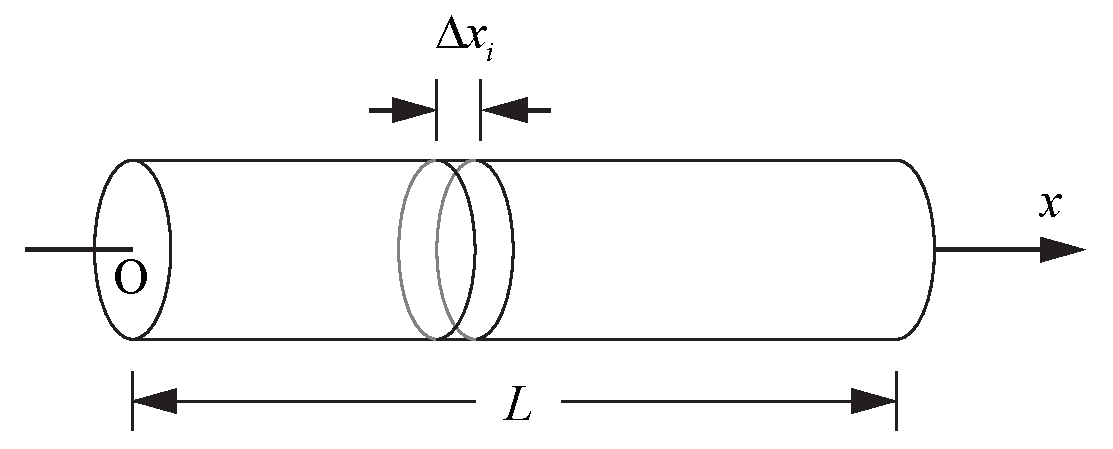
\includegraphics[width=9cm]{./figures/DefInt1.pdf}
\caption{密度不均匀的绳子}
\end{figure}

如果题目中,密度是恒定的,那么直接可以写出绳子的质量为 $m = LS\rho$. 但是题中 $\rho(x)$是关于 $x$ 的函数,所以我们要寻找另外的做法.假设绳子的密度变化是连续且“平滑”的,我们可以通过把绳子分割成 $n$ 小节(注意这些小节必须严格地首尾相接,不能有重合或者空隙).第 $i$ 节取 $x_i$ 到 $x_{i +1}$, 令其长度为 $x_{i + 1} - {x_i} = \Delta x_i$ 使每一个小节内,密度可以近似看成是恒定的,这样我们可以用 $\rho(\xi_i)\,\, (x_i \les \xi_i \les x_{i + 1})$ 来代替第 $i$ 节的密度,当每一节足够小时,可以认为 $\xi_i$ 在 $x_i \les \xi_i \les x_{i + 1}$ 约束下的取值并不会影响结果. 第 $i$ 小节的质量为
\begin{equation}
\Delta {m_i} = \rho (\xi_i)\Delta {x_i}S 
\end{equation}
所以总的质量用求和符号来表示,就是
\begin{equation}
m = \sum_{i = 1}^n \Delta m_i  \approx \sum_{i = 1}^n \rho(\xi_i)\Delta x_i S   = S \sum_{i = 1}^n \rho (\xi_i)\Delta x_i
\end{equation}
由于当 $n$ 取有限值时,上式并不精确成立,所以只能使用约等号,但是 $n$ 越大,约等号两边就越精确成立.这是极限的思想,用极限符号来表,就是
\begin{equation}
m = \lim_{n \to \infty } \sum_{i = 1}^n {\Delta {m_i}}  = \lim_{n \to \infty } \sum_{i = 1}^n \rho(\xi_i)\Delta {x_i}S   = S   \lim_{n \to \infty } \sum_{i = 1}^n \rho(\xi_i)\Delta {x_i}
\end{equation}
这种表达式在物理中反复出现,所以使用积分符号 $\int {} $ 用于代替极限和求和符号.另外把 ${\xi_i}$ 写成 $x$ (当 $n$ 趋近于无穷大时,参量 $i$ 和 $\Delta {x_i}$ 具体是多少就不重要了),把表示增量的 $\Delta $ 变为表示微小量的 $\dd$, 上式就写为
\begin{equation}
m = \int \dd{m}  = \int S\rho(x) \dd{x}  = S\int \rho(x) \dd{x}
\end{equation}
下面先看看 $\int \rho(x) \dd{x}$, 即 $\lim\limits_{n \to \infty } \sum\limits_{i = 1}^n \rho(\xi_i)\Delta {x_i}$的另一种理解.画出 $\rho (x)$图像.例如 $\rho(x) = x + 1$, 则 $\rho(\xi_i)\Delta {x_i}$可以表示左图的第 $i$ 个小长方形的面积, $\sum\limits_{i = 1}^n \rho(\xi_i)\Delta x_i$表示长方形面积之和.如果 $n$ 非常大且每个 $\Delta x_i$ 取得非常小,左图看起来就会像右图. 所以 $\int \rho(x) \dd{x}$ 可以用来表示右图阴影部分的面积.

\begin{figure}[ht]
\centering
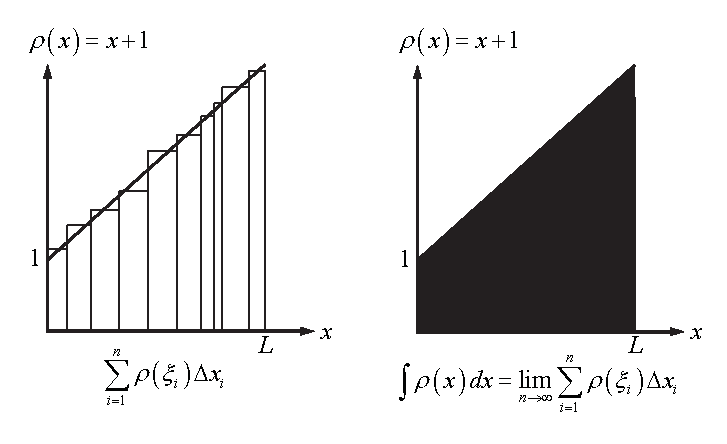
\includegraphics[width=12cm]{./figures/DefInt2.pdf}
\caption{定积分可以理解为曲线下面的面积, 并看做由无限多个无穷窄的矩形组成.} \label{DefInt_fig1} % 未完成:阴影用灰色会更好
\end{figure}

但 $\int \rho(x) \dd{x}$ 里面显然不包含 $0$ 和 $L$ 的信息,我们根据题目中的情况,说这个积分是“从 $0$ 积到 $L$”,其中 $0$ 是积分下限,$L$ 是积分上限.为了表示这个信息,把它写到积分号右边变为
\begin{equation}
\int_0^L \rho(x) \dd{x}
\end{equation}
这就是定积分的标准形式,但有时候为了书写方便,在不混淆的情况下可以把积分上下限省略.
\end{exam}

这样的写法是很形象的,可以想象,积分号就是函数的曲线需要积分的部分,下标的位置代表曲线的起点,上标代表曲线的终点.这样,物理中很多问题就可以用积分表示了.

要注意的是,根据上面积分的定义,如果曲线在 $x$ 轴的下方,面积应该表示成负值.但根据\autoref{DefInt_ex1} 的物理情景,可知密度不可能是负值.

至于计算积分的具体方法,比求导要复杂得多,甚至很多积分的结果不能用初等函数表示,只能表示为级数等形式.然而对于基本初等函数的积分,用牛顿-莱布尼兹公式\upref{NLeib} 即可马上求解.

\begin{exam}{求圆的面积}\label{DefInt_ex2}
在直角坐标系中, 圆的方程为 $x^2 + y^2 = R^2$, 上半圆的方程可看做 $y$ 关于 $x$ 的函数
\begin{equation}
y = f(x) = \sqrt{R^2 - x^2} \quad (x\in [-R,R])
\end{equation}
将该式定积分再乘以 2 即可得到圆的面积
\begin{equation}
S = 2\int_{-R}^{R} f(x) \dd{x} = 2\int_{-R}^{R} \sqrt{R^2 - x^2} \dd{x}
\end{equation}

我们还可以用另一种方法验证圆的面积公式. 把原划分成许多微小圆环, 由\autoref{Diff_ex2}\upref{Diff}, 每个微小圆环的面积为 $2\pi r\dd{r}$, 所以圆的面积可以用定积分表示为
\begin{equation}
S = \int_0^{R} 2\pi r\dd{r}
\end{equation}

以上两个定积分的结果都为 $\pi R^2$, 过程见 “牛顿—莱布尼兹公式\upref{NLeib}”的\autoref{NLeib_ex2}.
\end{exam}

\begin{exam}{球体的表面积}

\begin{figure}[ht]
\centering
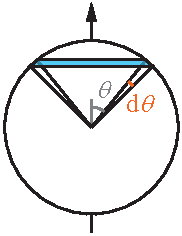
\includegraphics[width=3.2cm]{./figures/DefInt3.pdf}
\caption{将球的表面划分成许多细圆环, 每个对应的极角为 $\dd{\theta}$} \label{DefInt_fig3}
\end{figure}

以球心为原点建立球坐标系, 我们可以把球体的表面根据不同的 $\theta$ 划分成许多细圆环(如\autoref{DefInt_fig3}), 每个圆环的面积等于周长乘以宽度, 即
\begin{equation}\label{DefInt_eq9}
\dd{S} = 2\pi R\sin\theta \cdot R\dd{\theta}
\end{equation}
所以球的表面积可以用定积分记为
\begin{equation}
S = \int_0^{\pi} 2\pi R\sin\theta \cdot R\dd{\theta} = 2\pi R^2 \int_0^{\pi} \sin\theta \dd{\theta}
\end{equation}

虽然我们还不会计算这个定积分(见 “牛顿—莱布尼兹公式\upref{NLeib}”), 但我们现在可以用一种巧妙的方法来简化问题. 让我们来计算每个细圆环在极轴方向投影的长度. 我们不妨把极轴叫做 $z$ 轴, 则对某个细圆环有 $z = R\cos\theta$, 微分得 $\dd{z} = -R\sin\theta \dd{\theta}$, 将该式消去\autoref{DefInt_eq9} 中的 $\dd{\theta}$ 得
\begin{equation}
\dd{S} = -2\pi R\dd{z}
\end{equation}
这说明无论细圆环的位置如何, 其面积与其在 $z$ 轴投影的长度的比值恒为 $2\pi$. 至于上式中的负号, 是因为我们假设了正的 $\dd{\theta}$ 对应正的面积, 而正的 $\dd{\theta}$ 却对应负的 $\dd{z}$. 由于面积恒为正值, 我们可以取绝对值将负号去掉. 这样, 球的表面积就可以用定积分表示为
\begin{equation}
S = \int_{-R}^{R} 2\pi R\dd{z}
\end{equation}
由于被积函数是一个常数, 定积分的结果就是该常数乘以积分区间的长度即 $4\pi R^2$.
\end{exam}

\begin{exam}{球的体积}\label{DefInt_ex4}
要计算一个半径为 $R$ 的球体的体积, 可以将球划分为无限个薄球壳, 每个薄球壳的体积等于该球壳的表面积乘以厚度(见\autoref{Diff_ex2}\upref{Diff}), 即 $\dd{V} = 4\pi r^2 \dd{r}$. 所以球的体积可用定积分表示为
\begin{equation}
V = \int_0^R 4\pi r^2 \dd{r}
\end{equation}
同样由“牛顿—莱布尼兹公式\upref{NLeib}” 可得积分结果为 $4\pi R^3/3$.
\end{exam}
